% MUST be compiled using the --shell-escape tag. "pdflatex --shell-escape main.tex"

\documentclass{article}
\input{Preamble.tex}
\usepackage[utf8]{inputenc}
\usepackage{gnuplottex}
\usepackage{tkz-fct}
\usepackage{graphicx}
\graphicspath{ {./images/} }

\title{The Application and Investigation of Lissajous Curves}
\author{Alyssa Eckerman, Elias Little}
\date{May 2019}

\pgfplotsset{compat=1.13}
\begin{document}

\maketitle
\section{History}
Lissajous curves were names after Jules Antoine Lissajous. He was French mathematician and physicist who lived from 1822 to 1880. Lissajous studied waves, specifically related to tuning forks. He first explored with tuning forks and water and studying the waves it created. He then moved onto studying acoustic waves using reflected light from a mirror. This study using light in 1855 and figures it created is now known as the Lissajous curves. The apparatus that he build to study the waves, had two tuning forks placed at right angles with mirrors attached to them. The light is then shone on to the first tuning fork, reflecting on the second, and then lastly reflected onto the screen. Depending on the frequency of the tuning forks, the shape created on the screen changes.  Lissajous for his work on "optical observation of vibration", which affects astronomy, physics and other sciences, won the Lacaze Prize in 1873 \cite{JulesAntoineLissajous}.
\begin{figure}[h]
    \centering
    \includegraphics[scale=0.75]{Images/lissajous_obs.jpg}
    \cite{LissajousFigures}
    \caption{"Figure 1: Apparatus built by Lissajous using tuning forks to make Lissajous Curves."}
    \label{fig:my_label}
\end{figure}

Though Lissajous was given credit for these curves, and is most well known for them, Nathaniel Bowditch discovered the curves 1815. Nathaniel Bowditch was born in 1773 in Salem, Massachusetts. Bowditch had to self teach himself calculus, Latin and French due to needing to drop out of school at the age of ten to help his family. He went on to study mathematics, astronomy, and discovered the Bowditch curves - better known as the Lissajous curves now-leading to his fame in the scientific community around the world. Due to his only brief study of the curves, and not as in depth as that of Jules Antoine Lissajous, he is often forgotten as the original discoverer \cite{NathanielBowditch}.
\begin{figure}[h]
    \centering
    \includegraphics[scale=0.3]{Images/harmonograph.jpg}
    \cite{Harmpic}
    \caption{"Figure 3: Harmonograph."}
    \label{fig:my_label}
\end{figure}

In 1857, Hugh Blackburn, a Scottish mathematician, built the first harmonograph. A harmonograph either has a swinging pencil and or platform, by the means of several pendulums. By pushing the pendulums, one can create "undulating drawings". They are now mostly used for fun, and creating pretty images, as the friction created by the pendulums and the pen dampens the image \cite{Harmonograph}. They can still be analyzed mathematically, but the dampening needs to be accounted for.
\begin{figure}[h]
    \centering
    \includegraphics[scale=0.75]{Images/oscilloscope.jpg}\cite{Oscilloscope}
    \caption{"Figure 2: Oscilloscope creating a Lissajous Curve."}
    \label{fig:my_label}
\end{figure}


Lissajous curves can also be created by oscilloscopes, which were invented in 1897. By sending different signals along the X and Y-axis, the image created is that of a Lissajous curve. Using the oscilloscopes one can study the relationship between the frequency, phase, ratio, and amplitude, and the image created\cite{Oscilloscope}.
\newpage
Additionally there is the more modern way of creating and analyzing Lissajous curves through coded programs. Now online it is rather easy to find programs that you plug in all of the variables and it will show you the Lissajous curve that would be created like Figure 4. Furthermore on computers, and with more complex programming, one can create 3D Lissajous curves to analyze shown in Figure 5.

\begin{figure}[h]
    \centering
    \includegraphics[scale=0.3]{Images/lissajous.PNG}
    \cite{Onlinecurve}
    \caption{"Figure 4: Online program allowing you to plug in all of the variables."}
    \label{fig:my_label}
\end{figure}
\newpage
\begin{figure}[h]
    \centering
    \includegraphics[scale=1.5]{Images/3dcurve.jpg}
    \cite{3DCurve}
    \caption{"Figure 5: 3D Lissajous Curve."}
    \label{fig:my_label}
\end{figure}

\newpage
\section{Mathematical Components}
Lissajous curves are the result of two, or more, intersecting perpendicular sinusoidal curves. The most common occurrence of sinusoidal curves is in objects that exhibit simple harmonic motion, such as tuning forks or a pendulum as Jules-Antoine Lissajous did. Simple harmonic motion has been understood and researched for hundreds of years, and the equation can be found using Isaac Newton's second law. The equation for simple harmonic motion in a single direction is: \[x(t)=A \cos (\omega t-\varphi)\] Because a Lissajous curves consist of multiple instances of simple harmonic motion, they are mathematically represented as the following common paramaterization of the single direction formula: \[x=A \sin (a t+\delta), \quad y=B \sin (b t)\]
Changing the different components of the paramaterization affects the curve in different ways, from stretching to adding lobes. We will now go through how each variable affects the graph.

\subsection{Phase Shift: $\delta$}
The easiest way to understand these changes is visually. Below is a graph showing how phase increasing phase shift, moving clockwise, affects the curve described by the equation $x = \sin(2\pi t + \delta), \quad y = \sin(2\pi t)$. One interesting note on the phase shift, is that if you picture the curve as being in three dimensions, the phase shift then appears to rotate the curve either vertically or horizontally depending on the $\frac{a}{b}$ ratio, which will be discussed further below.
\begin{figure}[h]
    \centering
    \includegraphics[scale=0.2]{Images/PhaseShift.png}
    \cite{PhaseShift}
    \caption{"Figure showing several Lissajous figures for different phase delays."}
    \label{fig:my_label}
\end{figure}
\newpage
\subsection{Amplitude: $A, B$}
In the single direction simple harmonic motion equation, these variables represent the magnitude of the motion. They act similarly here, but for their respective directions. The ratio $\frac{A}{B}$ represents the width to height ratio. \\ \\

\textbf{Changing A:}
\begin{center}
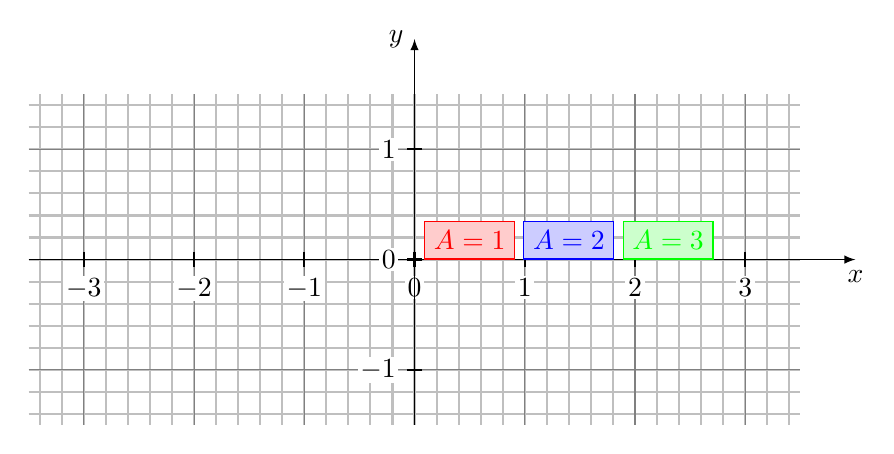
\begin{tikzpicture}[scale=1.4][h]
    \tkzInit[xmin=-3.5,xmax=3.5,xstep=1,ymin=-1.5,ymax=1.5,ystep=1]
    \tkzGrid[sub]
    \tkzAxeX[step=1]
    \tkzAxeY[step=1]
    \tkzFctPar[color = red, samples=200,domain=-pi:pi]{sin(t)}{sin(t+pi/2)}
    \tkzText[draw, above, color = red, fill = red!20](0.5,0){$A=1$}
    \tkzFctPar[color = blue, samples=200,domain=-pi:pi]{2*sin(t)}{sin(t+pi/2)}
    \tkzText[draw, above, color = blue, fill = blue!20](1.4,0){$A=2$}
    \tkzFctPar[color = green, samples=200,domain=-pi:pi]{3*sin(t)}{sin(t+pi/2)}
    \tkzText[draw, above, color = green, fill = green!20](2.3,0){$A=3$}
\end{tikzpicture}
\end{center}

\newpage
\textbf{Changing B:}
\begin{center}
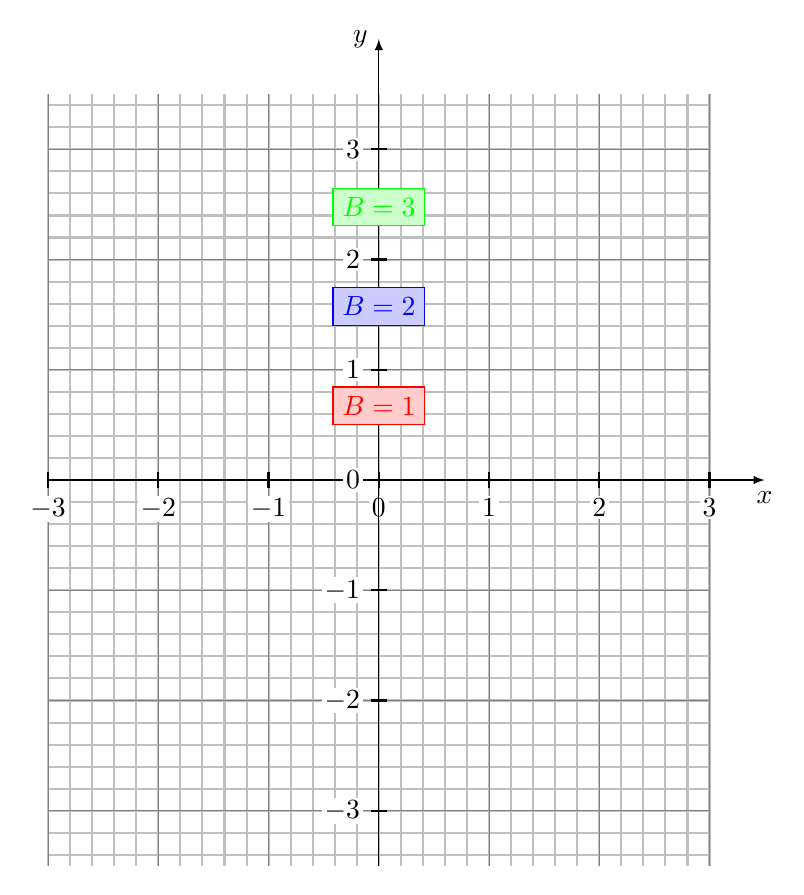
\begin{tikzpicture}[scale=1.4][h]
    \tkzInit[xmin=-3,xmax=3,xstep=1,ymin=-3.5,ymax=3.5,ystep=1]
    \tkzGrid[sub]
    \tkzAxeX[step=1]
    \tkzAxeY[step=1]
    \tkzFctPar[color = red, samples=200,domain=-pi:pi]{sin(t)}{sin(t+pi/2)}
    \tkzText[draw, above, color = red, fill = red!20](0,0.5){$B=1$}
    \tkzFctPar[color = blue, samples=200,domain=-pi:pi]{sin(t)}{2*sin(t+pi/2)}
    \tkzText[draw, above, color = blue, fill = blue!20](0,1.4){$B=2$}
    \tkzFctPar[color = green, samples=200,domain=-pi:pi]{sin(t)}{3*sin(t+pi/2)}
    \tkzText[draw, above, color = green, fill = green!20](0,2.3){$B=3$}
\end{tikzpicture}
\end{center}

\subsection{Lobes: $a, b$}
These variables are perhaps the most interesting of the variables. The most obvious affect of changing these variables is the number of lobes. $a$ determines the number of vertical lobes, and $b$ determines the number of horizontal lobes. For the ratio $\frac{a}{b} = 1$, the curve produced is an ellipse, or, depending on the phase shift, a circle or line. Higher ratios result in more complex curves. As long as the ratio $\frac{a}{b}$ is rational, it will produce a closed figure, otherwise it will never loop back around. Below are some examples with different $\frac{a}{b}$ ratios.

\begin{figure}[h]
\begin{tikzpicture}[scale=0.8][h]
    \tkzInit[xmin=-2,xmax=2,xstep=1,ymin=-2,ymax=2,ystep=1]
    \tkzAxeX[step=1]
    \tkzAxeY[step=1,above]
    \tkzFctPar[color = red, samples=200,domain=0:2*pi]{sin(5*t+pi/4)}{sin(3*t)}
    \tkzText[draw, text width=2.6cm, above, left, color = red, fill = red!20](-2,2){$x = \sin(5t+\frac{\pi}{4}) \\ y = \sin(3t)$}
\end{tikzpicture}
\begin{tikzpicture}[scale=0.8][h]
    \tkzInit[xmin=-2,xmax=2,xstep=1,ymin=-2,ymax=2,ystep=1]
    \tkzAxeX[step=1]
    \tkzAxeY[step=1,above]
    \tkzFctPar[color = blue, samples=200,domain=0:8*pi]{sin(pi*t+pi/4)}{sin(2*t)}
    \tkzText[draw, text width=2.6cm, above, left, color = blue, fill = blue!20](-2,2){$x = \sin(\pi t+\frac{\pi}{4}) \\ y = \sin(2t)$}
\end{tikzpicture}
\begin{tikzpicture}[scale=0.8][h]
    \tkzInit[xmin=-2,xmax=2,xstep=1,ymin=-2,ymax=2,ystep=1]
    \tkzAxeX[step=1]
    \tkzAxeY[step=1,above]
    \tkzFctPar[color = green, samples=200,domain=0:2*pi]{sin(4*t)}{sin(3*t)}
    \tkzText[draw, text width=2.6cm, above, left, color = green, fill = green!20](-2,2){$x = \sin(4t) \\ y = \sin(3t)$}
\end{tikzpicture}
\hfill\begin{tikzpicture}[scale=0.8][h]
    \tkzInit[xmin=-2,xmax=2,xstep=1,ymin=-2,ymax=2,ystep=1]
    \tkzAxeX[step=1]
    \tkzAxeY[step=1,above]
    \tkzFctPar[color = purple, samples=200,domain=0:2*pi]{sin(t+pi/2)}{sin(3*t)}
    \tkzText[draw, text width=2.6cm, above, left, color = purple, fill = purple!20](-2,2){$x = \sin(t+\frac{\pi}{2}) \\ y = \sin(3t)$}
\end{tikzpicture}
\end{figure}

Many people draw parallels between these figures and three-dimensional knots, which is a valid connection. Many knots when projected into a plane are Lissajous curves, these are called Lissajous knots.

\newpage
\section{Arc Length}
\subsection{Ideal Curves}
One of the main concepts we learned this year in Multivariable Calculus, is finding the arc length of a curve. The formula for finding arc length of a curve is: \[\int_{a}^{b}\|\vec{c}^{\ \prime}(t)\|dt \text{ for } \vec{c}:[a, b] \rightarrow \R^{2}\]

We already know the paramaterization for Lissajous curves, so we can solve for $\|\vec{c}^{\ \prime}(t)\|$ through a short series of steps. We begin with our paramaterization: \[\vec{c}(t) = [A\sin(at+\delta),\ B\sin(bt)].\] From there, by differentiating both variables with respect to $t$, we see that \[\vec{c}^{\ \prime}(t) = [Aa\cos(at+\delta),\  Bb\cos(bt)].\] Then we can use Pythagoras' theorem to calculate the magnitude of c-prime. Doing so gives us: \[\|\vec{c}^{\ \prime}(t)\| = \sqrt{(Aa\cos(at+\delta))^2 + (Bb\cos(bt))^2}.\] Our integral now looks like this: \[\int_{t_0}^{t_f}\sqrt{(Aa\cos(at+\delta))^2 + (Bb\cos(bt))^2}\ dt\].

Before we can plug in our variables and evaluate, we need to solve for our bounds. Our lower bound is rather trivial, starting at $t=0$ unless special circumstances call for otherwise. Our upper bound is slightly more complicated. We can choose any time $t>0$, to find the arc length of the curve traced out until then, but eventually the curve will repeat itself. We can solve for what time the curve returns to it's initial position, which will allow us to find the arc length of the entire curve. To do so, we set the equation for $x$ and $y$ equal to their value at $t=0$: \[A\sin(at+\delta) = A\sin(\delta) \\ B\sin(bt) = 0.\] From the y equation, we know that $bt_f$ must be a multiple of $2\pi$. Let's look at an example: \[x=3\sin(4t),\ y=2\sin(3t).\]
\begin{center}
\begin{tikzpicture}[scale=0.8][h]
    \tkzInit[xmin=-4,xmax=4,xstep=1,ymin=-3,ymax=3,ystep=1]
    \tkzAxeX[step=1]
    \tkzAxeY[step=1,above]
    \tkzFctPar[color = purple, samples=200,domain=0:2*pi]{3*sin(4*t)}{2*sin(3*t)}
\end{tikzpicture}
\end{center}

In this example $t_f = 2\pi$, which means we can now integrate. For brevity, I will skip the steps for finding $\|\vec{c}^{\ \prime}(t)\|$ for this specific example and jump straight to the integral: \[\int_{0}^{2\pi}\sqrt{(12\cos(4t))^2 + (6\cos(3t))^2}\ dt \approx 56.2578.\]

\subsection{Real Curves}
The above work was for ideal Lissajous curves, but in the real world when we create the curves using harmonographs there's friction, which causes dampening in the curve. When we have dampening, we have to add a dampening factor to our parametric equations, when we do so, our new equations look like: \[x=A \sin (a t+\delta)e^{-dt}, \quad y=B \sin (b t)e^{-dt}\]

\begin{figure}[h]
\caption{Example of a Lissajous curve with and without dampening}
\begin{tikzpicture}[scale=0.8][h]
    \tkzInit[xmin=-2,xmax=2,xstep=1,ymin=-2,ymax=2,ystep=1]
    \tkzAxeX[step=1]
    \tkzAxeY[step=1,above]
    \tkzFctPar[color = red, samples=200,domain=0:2*pi]{sin(4*t)}{sin(3*t)}
    \tkzText[draw, text width=2.6cm, above, left, color = red, fill = red!20](-2,2){$x = \sin(4t) \\ y = \sin(3t)$}
\end{tikzpicture}
\begin{tikzpicture}[scale=0.8][h]
    \tkzInit[xmin=-2,xmax=2,xstep=1,ymin=-2,ymax=2,ystep=1]
    \tkzAxeX[step=1]
    \tkzAxeY[step=1,above]
    \tkzFctPar[color = blue, samples=1000,domain=0:100]{sin(4*t)*exp(-0.01*t)}{sin(3*t)*exp(-0.01*t)}
    \tkzText[draw, text width=3cm, above, left, color = blue, fill = blue!20](-1.5,2){$x = \sin(4t)e^{-0.01t} \\ y = \sin(3t)e^{-0.01t}$}
\end{tikzpicture}
\end{figure}
\newpage

Using this new paramaterization, we can recalculate the arc length. Following the same process as above, we can find that \[\|\vec{c}^{\ \prime}(t)\| = \sqrt{ (Aa\cos(at+\delta)e^{-dt} - dA\sin(at+\delta)e^{-dt})^2 +  (Bb\cos(bt)e^{-dt} - dB\sin(Bb)e^{-dt})^2}\] At this point before we solved for our bounds to integrate over, however because of the dampening there is no time where the curve returns to it's original position. In theory, the curve would continue forever without stopping, but calculus is all about evaluating at infinities, so we can still evaluate the integral as $t\rightarrow \infty$: \[\int_{0}^{\infty}\sqrt{ (Aa\cos(at+\delta)e^{-dt} - dA\sin(at+\delta)e^{-dt})^2 +  (Bb\cos(bt)e^{-dt} - dB\sin(bt)e^{-dt})^2}\ dt\] If we use the same example as above, but with a dampening factor of $d=-0.01$, our final integral to evaluate is: \[\int_{0}^{\infty}\sqrt{ (12\cos(4t)e^{-0.01t} - 0.03\sin(4t)e^{-0.01t})^2 +  (6\cos(3t)e^{-0.01t} - 0.02\sin(3t)e^{-0.01t})^2}\ dt\ \approx 895.37\]

\newpage
\section{Path Integral}
For ideal Lissajous curves, the paramaterization is also a path in $\R^2$. As a result, we can take path integrals. We essentially did this to find the arc length. The equation for a path integral is: \[\oint_{C}f(\vec{c}(t))\|\vec{c}^{\ \prime}(t)\|dt\] When calculating the arc length we had essentially set $f(\vec{c}(t)) = 1$. Which creates a path integral where the height at every point is equal to $1$, and thus the final value is the same as the arc length. However, we aren't limited to solely finding the arc length. For example, we could take a path integral over any function $f(x,y)$. I provide an example below:
\begin{center}
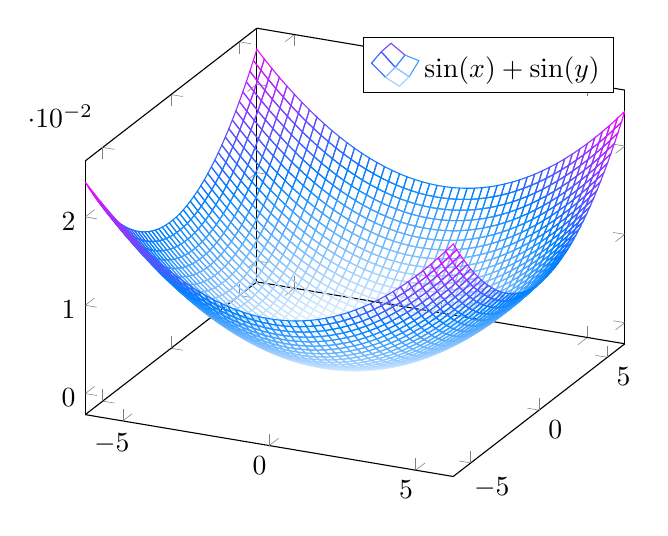
\begin{tikzpicture}[scale=1][h]
\begin{axis}[
    colormap/cool,
]
\addplot3[
    mesh,
    samples=50,
    domain=-2*pi:2*pi,
]
{sin(x)^2+sin(y)^2};
\addlegendentry{$\sin(x)+\sin(y)$}
\end{axis}
\end{tikzpicture}
\end{center}

\newpage
\section{Contributions}
\subsection{Choice of Topic}
We both really wanted to do something related to building, as we both are in robotics, and spend a lot of our free time making things. Alyssa really likes more hands on math, as it is easier to visualize what is going and understand the material. Not to mention, that we both think the images that are created are really spectacular.

When you look up harmonographs, often what comes up is Lissajous curves, which when dampening is taken into consideration, can describe the images made. Which is why we spent a lot of time researching Lissajous curves, and talk a lot about it. However, we also realized that due to the paramaterization of Lissajous curves, one can use line integrals to figure out the arc length of the image. Furthermore you can use a line integral to find the surface area of the image created.

\subsection{Paper}
\begin{itemize}
\item Initial Research -Alyssa
\item Rough Draft -Elias and Alyssa
\item History -Alyssa
\item Mathematical components -Elias
\item Arc Length and Surface Integral -Elias
\item Contributions -Alyssa
\item Conclusion -Alyssa
\end{itemize}
\subsection{Presentation}
\begin{itemize}
\item Rough Draft -Elias
\item History -Alyssa
\item Mathematical Components -Alyssa
\item Arc Length and Curvature -Elias
\item Our Harmonograph -Alyssa
\end{itemize}
\subsection{Harmonograph}
\begin{itemize}
\item Initial Research/Design -Alyssa
\item Materials -Alyssa
\item Built -Elias and Alyssa at Elias' shop
\item Transportation -Elias
\end{itemize}

\section{Conclusion}
Lissajous curves were first discovered over 200 years ago, and the way that we study them has continually evolved. They affect our style of art, our engineering, and our study of astronomy and physics. Lissajous curves can be made both digitally-oscilloscopes, online programs- and physically-Lissajous apparatus, and harmanographs. The images created can be analyzed through the parameterization of the Lissajous curves, as well as the line integrals. Though there is a difference between ideal and the real world, meaning that dampening would need to be considered in the calculations for the curves created by that of physical models. 

\newpage
\begin{thebibliography}{9}
%\bibitem{latexcompanion}
%Michel Goossens, Frank Mittelbach, and Alexander Samarin.
%\textit{The \LaTeX\ Companion}.
%Addison-Wesley, Reading, Massachusetts, 1993.
\bibitem{Harmonograph}
“Beautiful Curves: The Harmonograph.” \textit{Fronkonstin}, 26 Sept. 2016, \texttt{fronkonstin.com/2014/10/13/beautiful-curves-the-harmonograph/}

\bibitem{LissajousFigures}
Greenslade, Thomas  B. “Lissajous Figures.” \textit{Instruments for Natural Philosophy}, \texttt{physics.kenyon.edu/EarlyApparatus/Oscillations\_and\_Waves/Lissajous\_Figures/
Lissajous\_Figures.html.}

\bibitem{JulesAntoineLissajous}
“Jules Antoine Lissajous (1822--1880) --- Historical Sketch.” \textit{Hardy Calculus,}
\texttt{hardycalculus.com/calcindex/IE\_lissajous.htm.}

\bibitem{PhaseShift}
Krishnavedala. "Figure showing several Lissajous figures for different phase delays."
\textit{Wikipedia}, Wikipedia, 20 Aug. 2014, \texttt{https://en.wikipedia.org/wiki/Lissajous\_curve\#/media/File:Lissajous\_phase.svg}

\bibitem{Onlinecurve}
“Lissajous Curves.” \textit{Lissajous Curves | Academo.org - Free, Interactive, Education.},\texttt{ academo.org/demos/lissajous-curves/}

\bibitem{Oscilloscope}
“Lissajous Figure.” \textit{Encyclopaedia Britannica}, 20 July 1998, \texttt{www.britannica.com/science/Lissajous-figure}

\bibitem{NathanielBowditch}
“Nathaniel Bowditch (1773--1838) --- Historical Sketch.” \textit{Hardy Calculus}, \texttt{hardycalculus.com/calcindex/IE\_bowditch.htm}

\bibitem{Harmpic}
Sims, Karl. “Harmonograph.” \textit{Karl Sims}, www.karlsims.com/harmonograph/

\bibitem{3DCurve}
Trott, Michael. “3D Lissajous Curve with Avoided Intersections.”\textit{Wolfram Demonstrations Project}, demonstrations.wolfram.com/

\end{thebibliography}
\end{document}
